\section{Work Flow Diagram}
\label{dsePPWFD}
The work flow diagrams are represented in figures \ref{wfdbase}, \ref{wfdmid} and \ref{wfdfinal} (pp. \pageref{wfdbase} - \pageref{wfdfinal}). They have been broken up into three parts in order to logically represent the 3 major milestones.

%\newpage
\begin{figure}[H]
\begin{center}
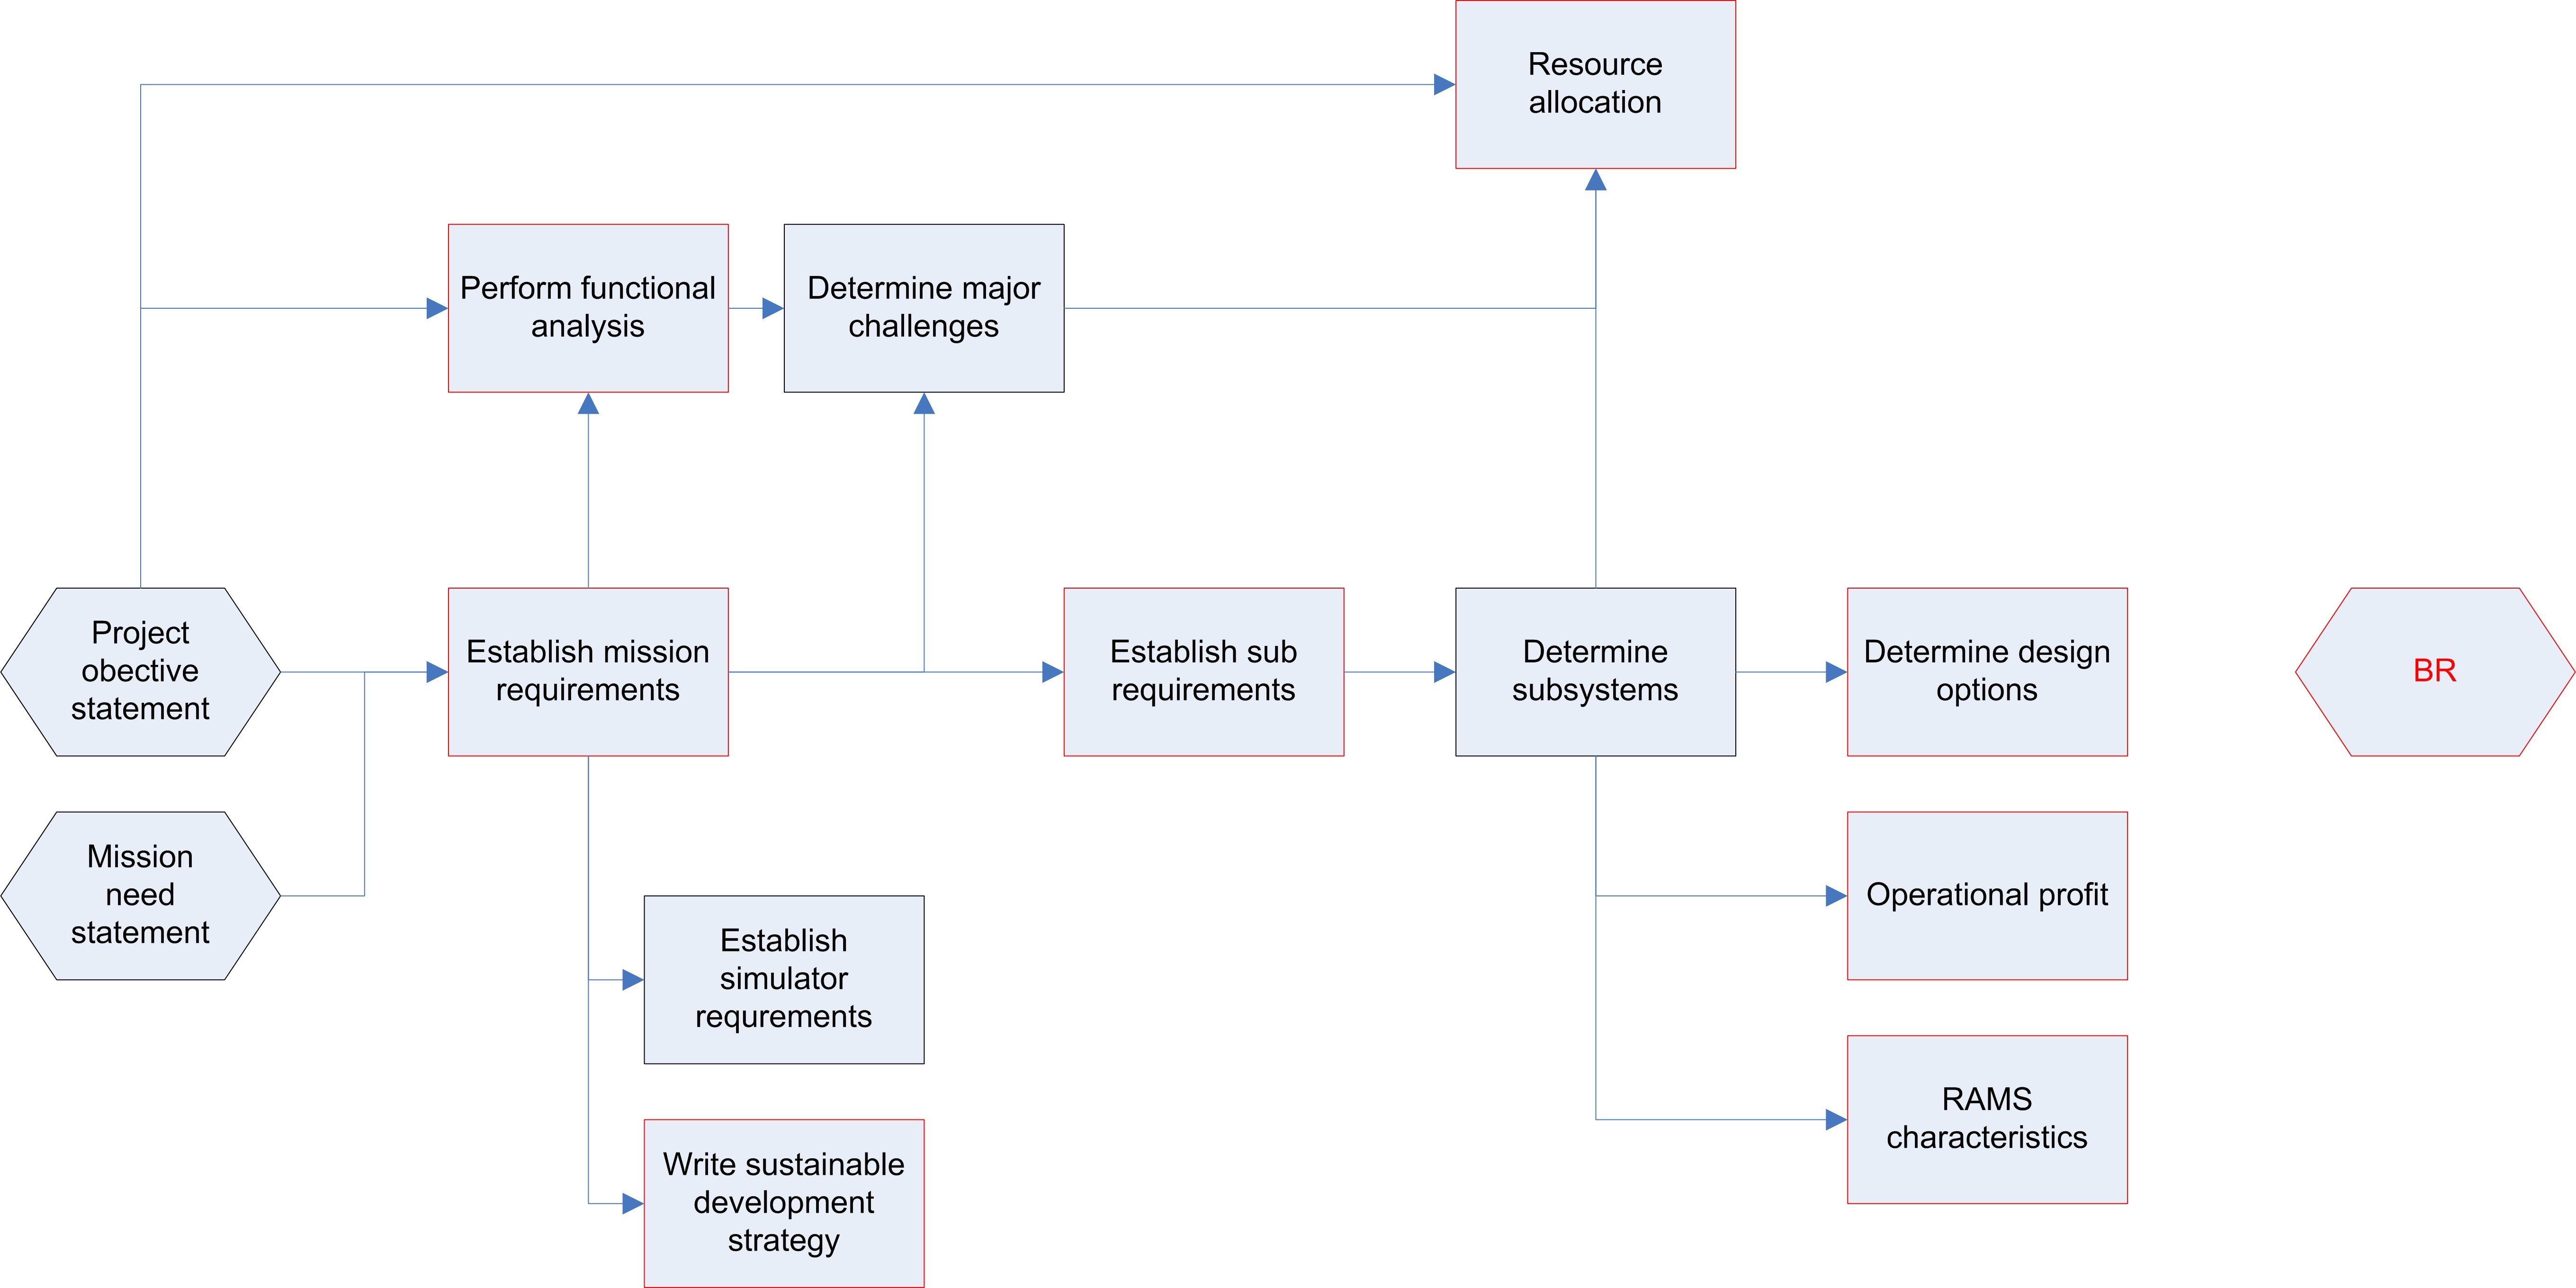
\includegraphics[width=1.2\textwidth, angle=90]{chapters/img/Workflow_diagram_BR.jpg}
\end{center}
\caption{Work flow diagram up until the Baseline review. Boxes in red lead to the BR.}
\label{wfdbase}
\end{figure}

%\newpage
\begin{figure}[H]
\begin{center}
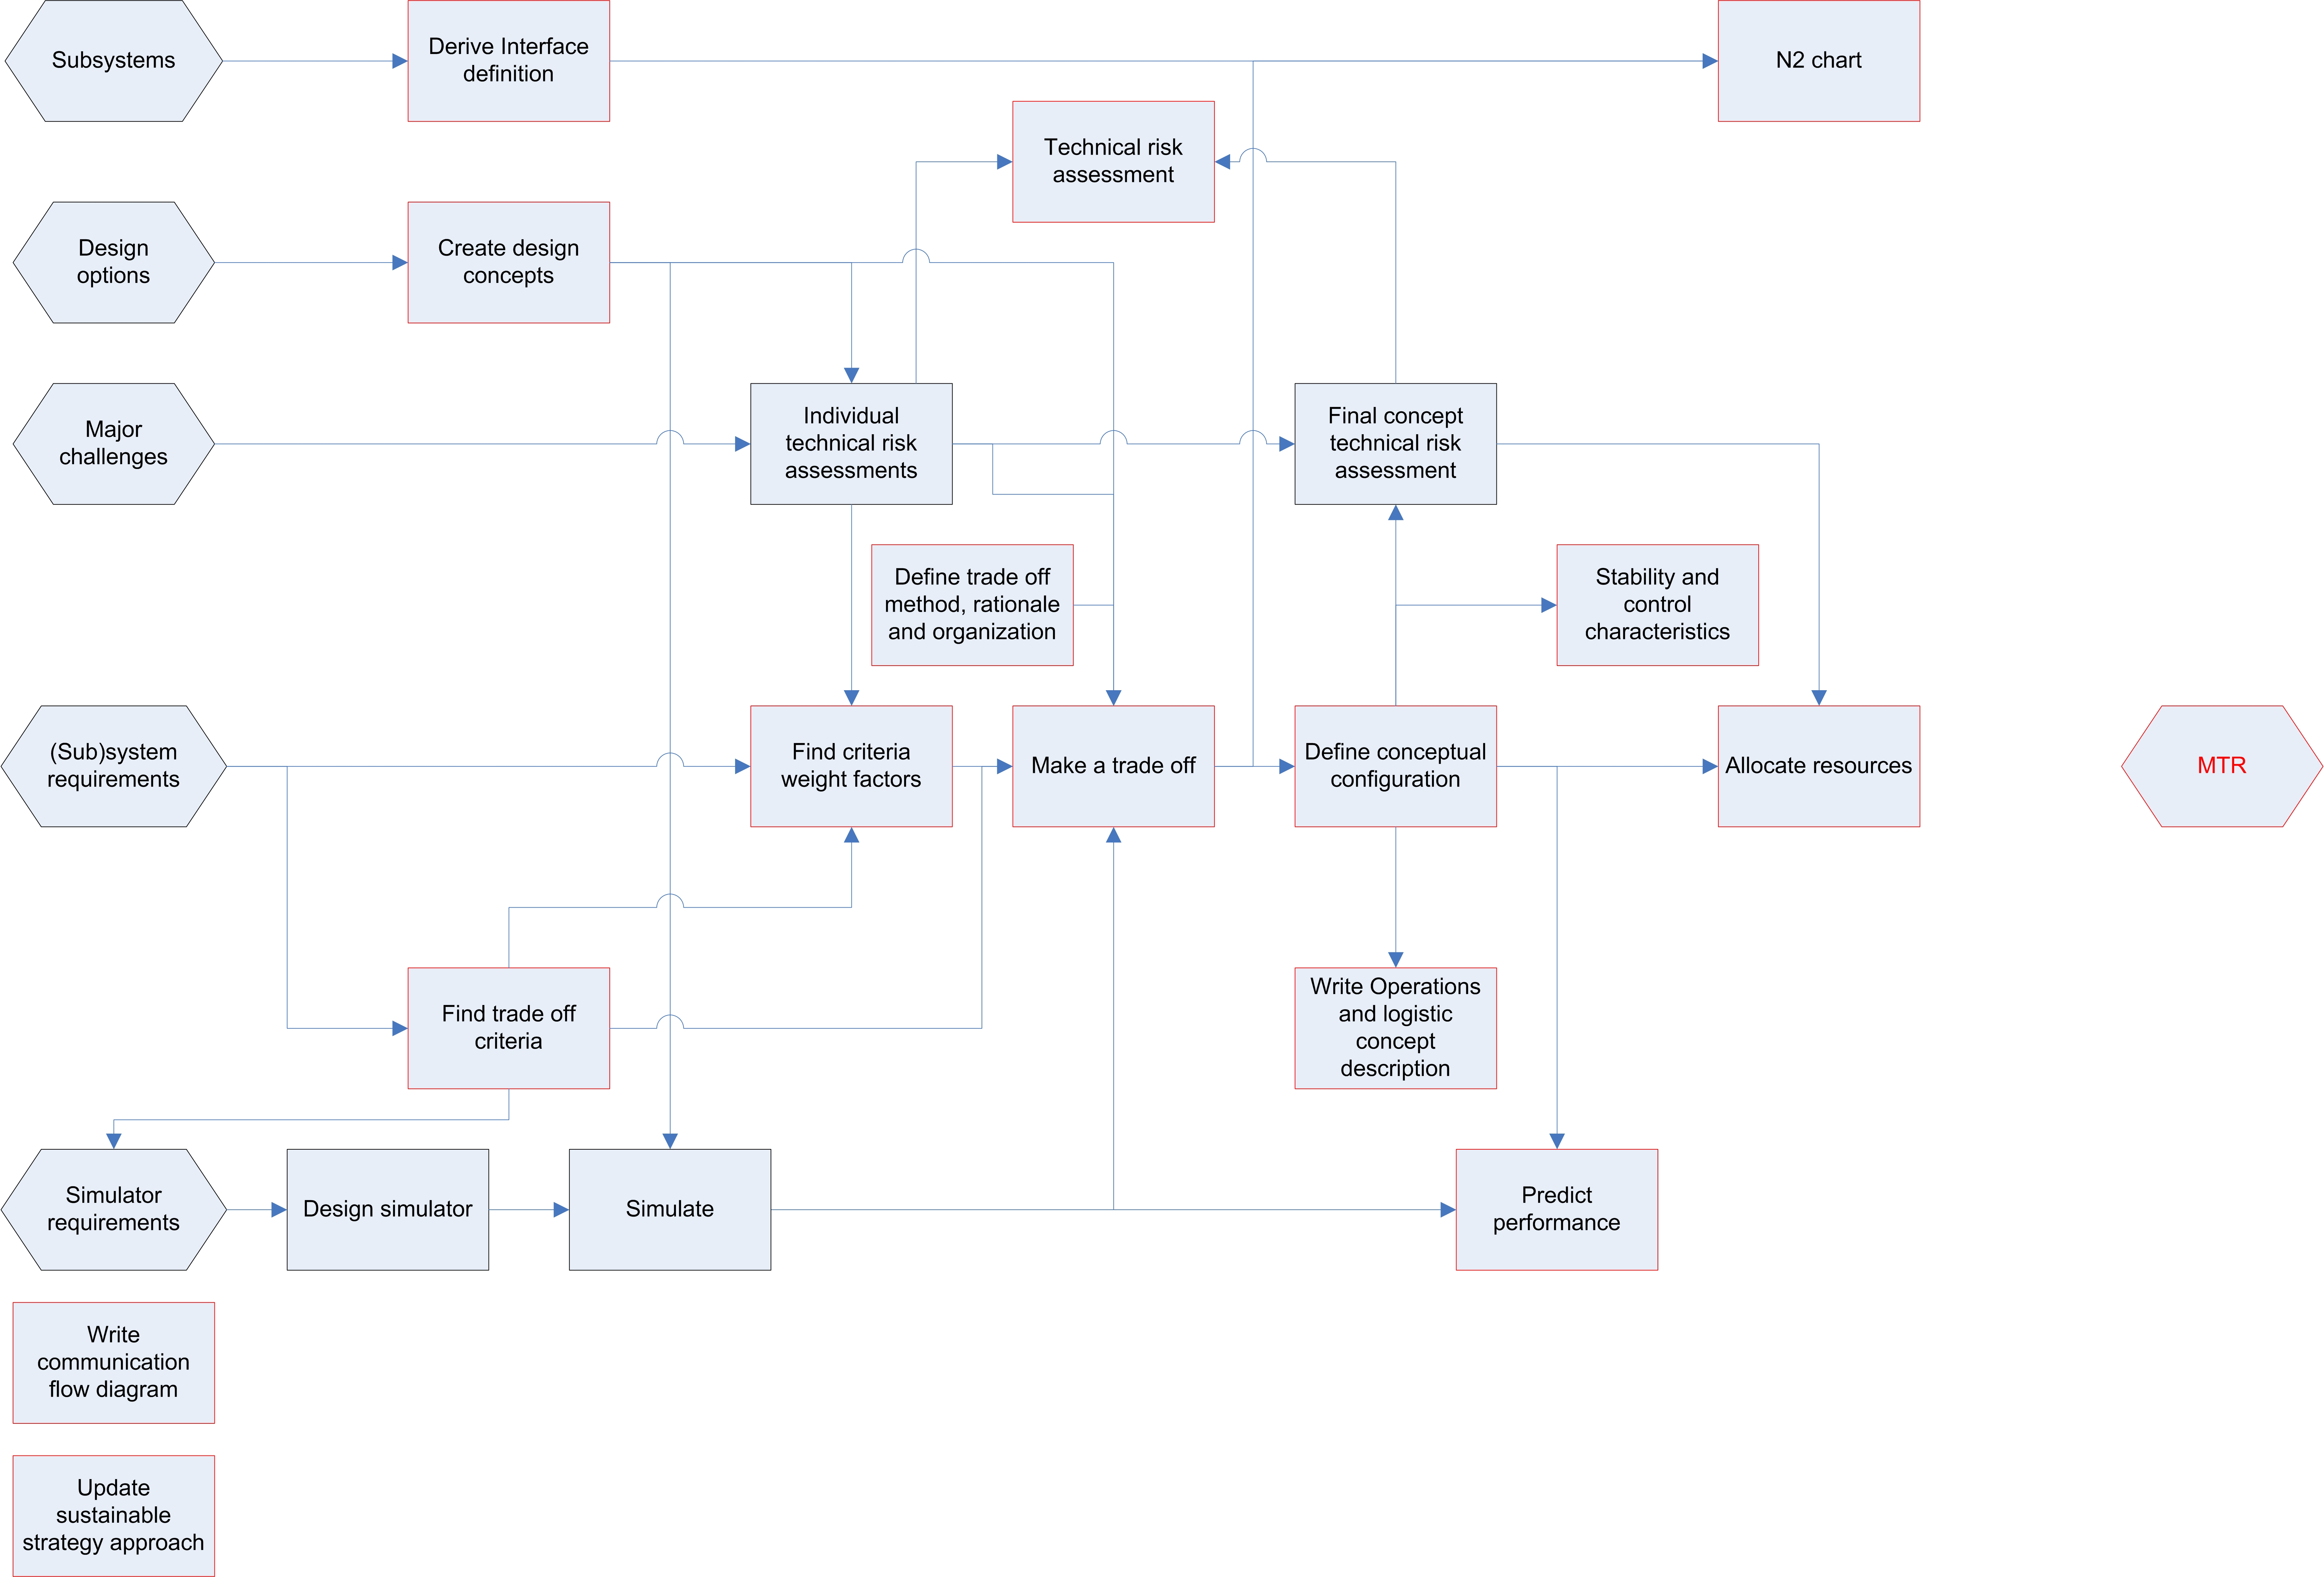
\includegraphics[width=1.2\textwidth, angle=90]{chapters/img/Workflow_diagram_MTR.jpg}
\end{center}
\caption{Work flow diagram up until the Mid term review. Boxes in red lead to the MTR.}
\label{wfdmid}
\end{figure}

%\newpage
\begin{figure}[H]
\begin{center}
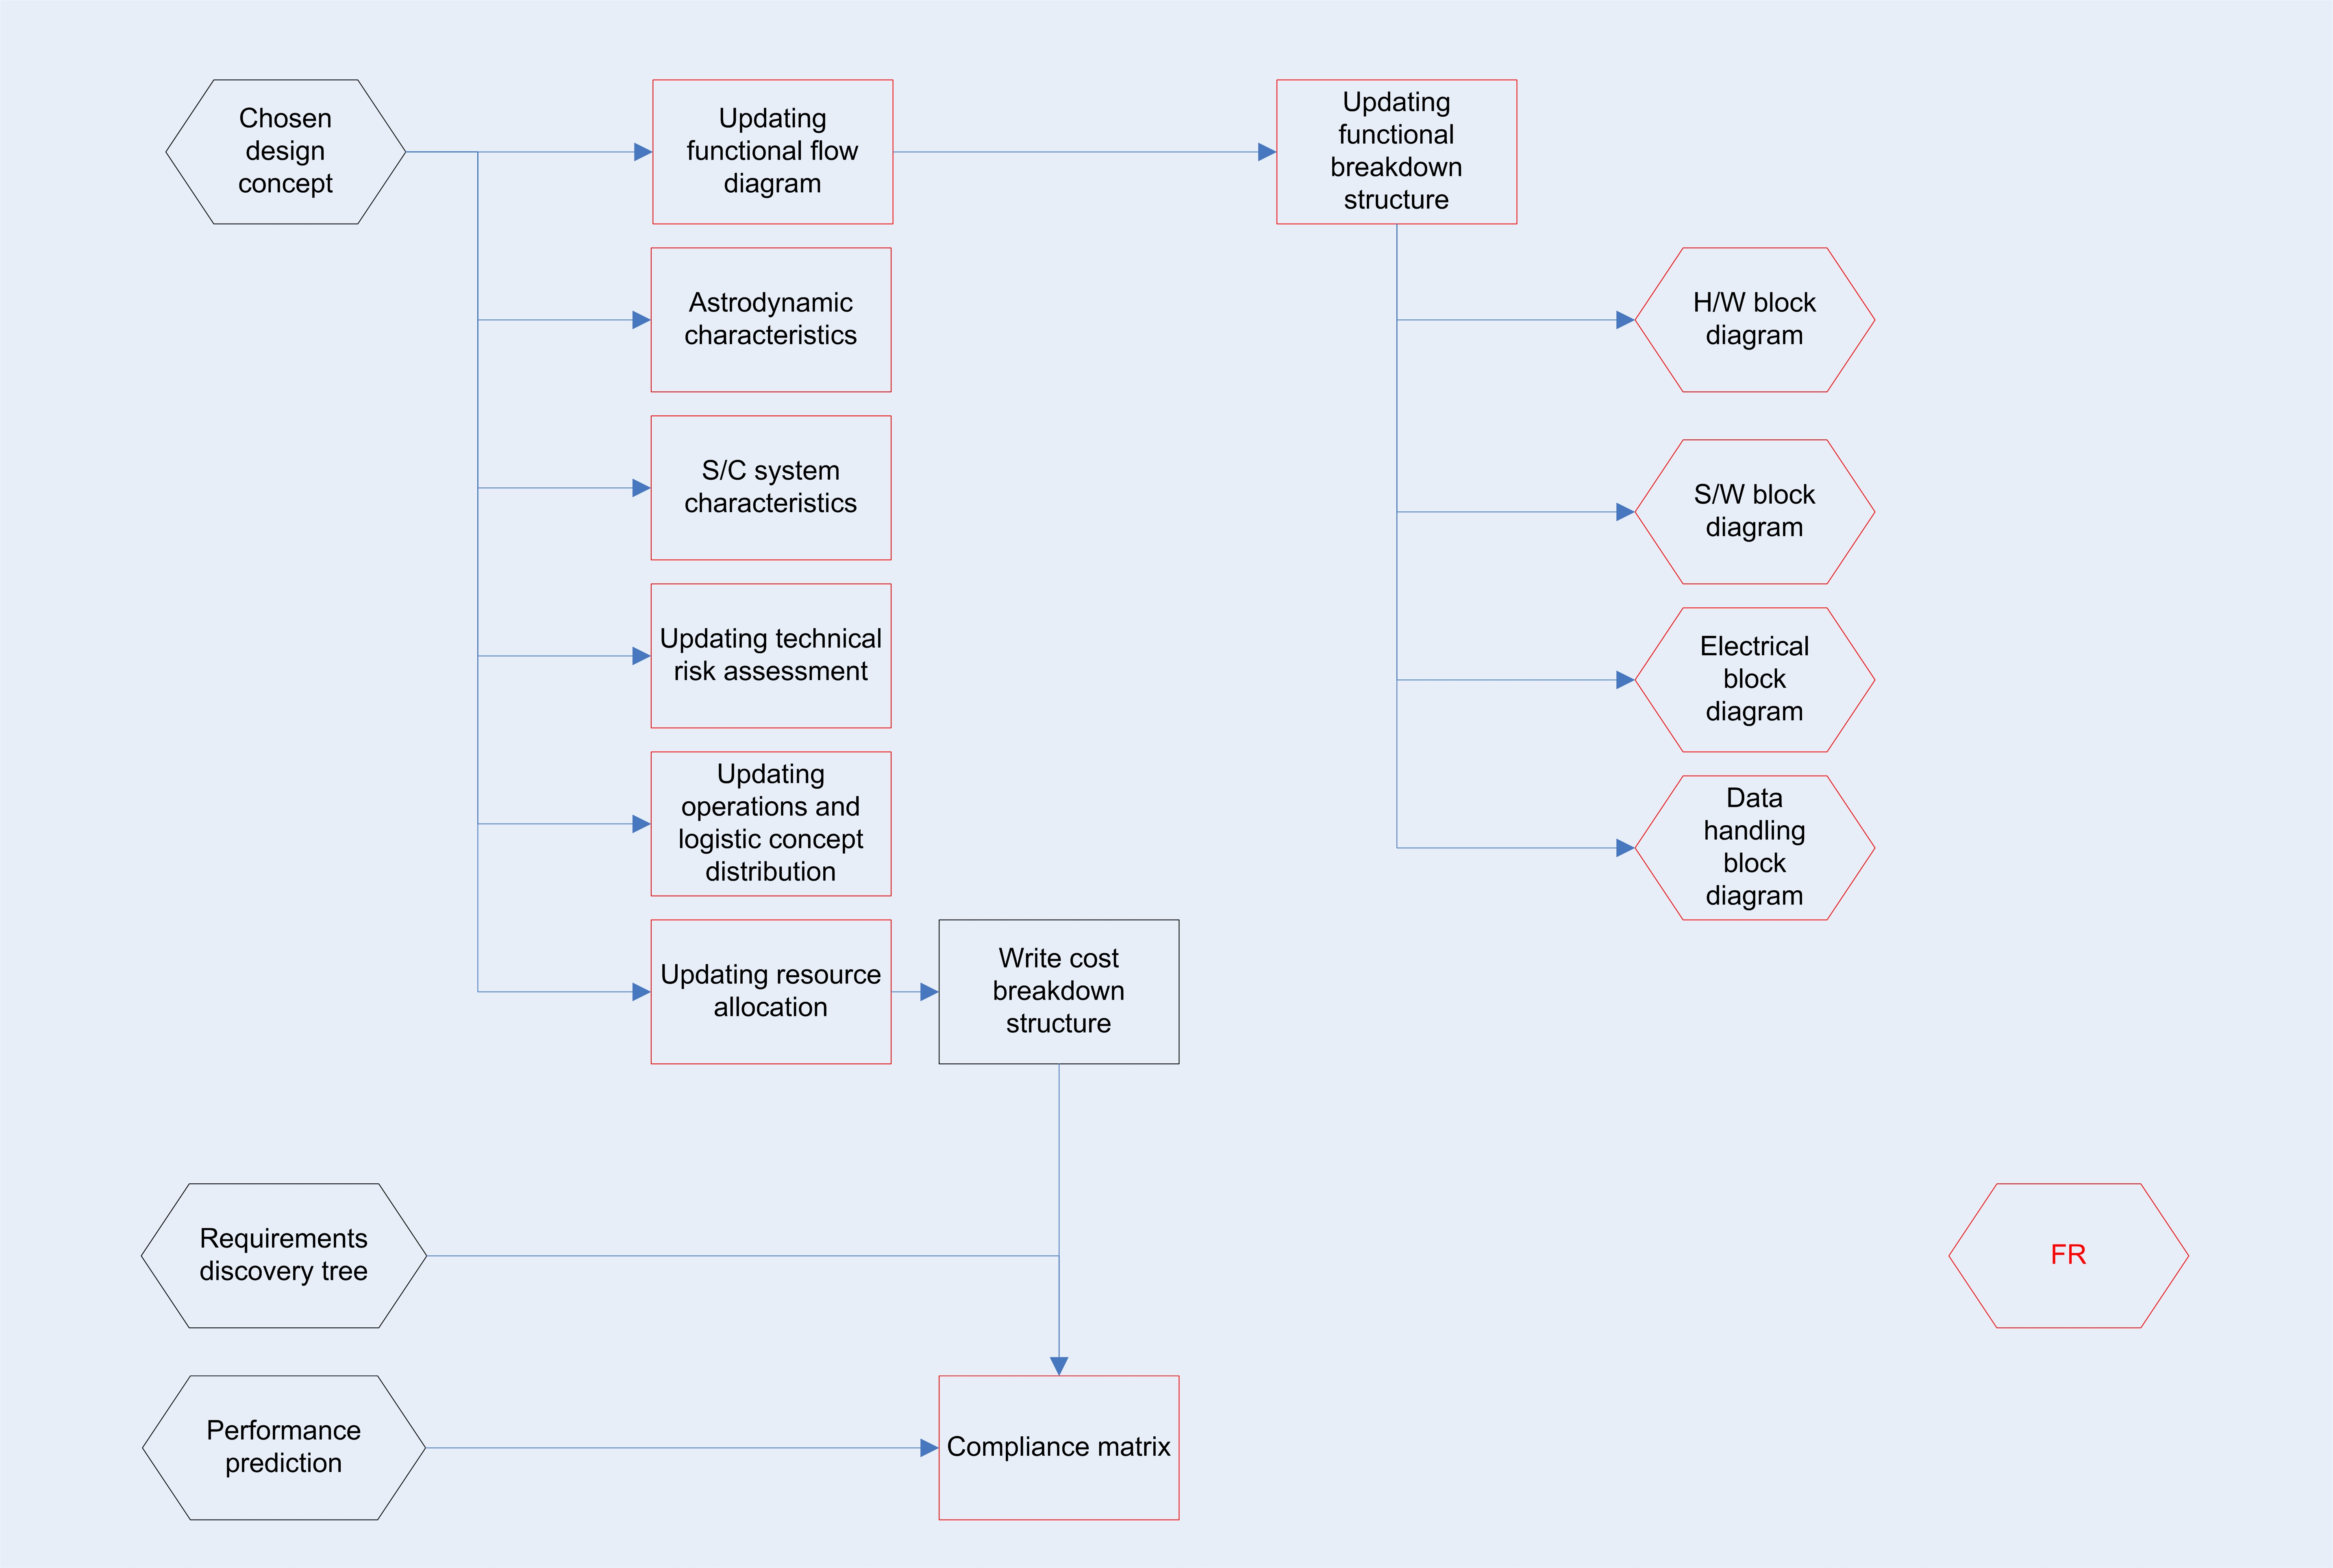
\includegraphics[width=1.2\textwidth, angle=90]{chapters/img/Workflow_diagram_FR.jpg}
\end{center}
\caption{Work flow diagram up until the Final review. Boxes in red lead to the FR.}
\label{wfdfinal}
\end{figure}